 \subsection{Extracción de características}
    Esta fase iba dividida en dos secciones, una para la estimación del tamaño de ventana y otra dedicada a la extracción de las características de la señal EMG.
    Todas las gráficas asociadas a cada una de las características pueden ser consultadas en el Anexo.(Ver \ref{anexo})

    Con respecto a la estimación del tamaño de ventana de cada repetición, a continuación se muestra una captura de pantalla sobre dicha resolución al problema:
    
    \begin{figure}[ht]
    \centering
    \includegraphics[scale=0.3]{imagenes/activación s1 serie 1 dia 1.png}
    \caption{ s1 serie 1 día 1: Ejemplo de activación muscular}
    \label{fig:s1 serie 1 dia 1}
    \end{figure}
    
    Otra funcionalidad que debe ser mostrada fue el análisis de todos los archivos de EMG disponibles, para descartar aquellos con mucho ruido o poca información. Aquí tenemos un ejemplo:
    
    \begin{figure}[ht]
    \centering
    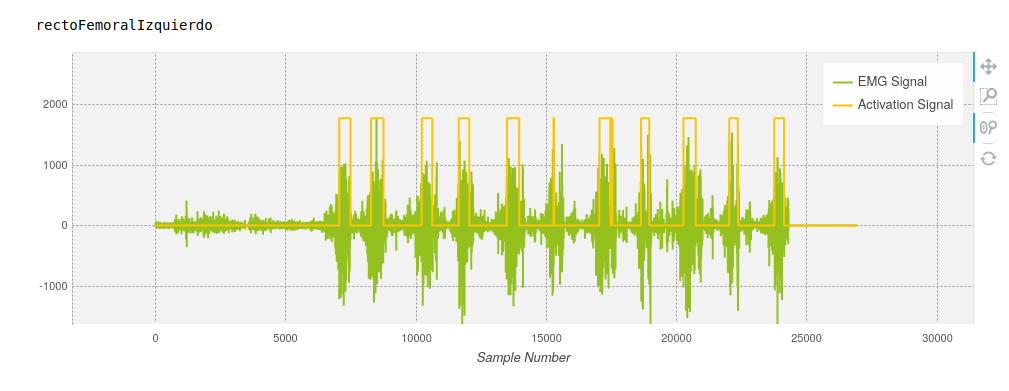
\includegraphics[scale=0.4]{imagenes/s3 serie 2 dia 2.png}
    \caption{ s3 serie 2 día 2: Ejemplo de activación muscular}
    \label{fig:s1 serie 1 dia 1 error}
    \end{figure}
    
    Como se puede apreciar, en este archivo de EMG, solo había registradas 11 repeticiones, por lo que no es válido para nuestro estudio.
    
    
    \subsection{Procesamiento de datos: Especificidad de los clasificadores}
    Esta sección va dedicada a mostrar cada uno de los archivos de entrenamiento-testeo utilizados para el estudio. Hay que recordar que de cada uno de ellos, se sacarán 3 con el RFECV, cada uno con un número diferente de características.
    \subsubsection{Canal 1}
        
        \begin{figure}[!ht]
            \centering
            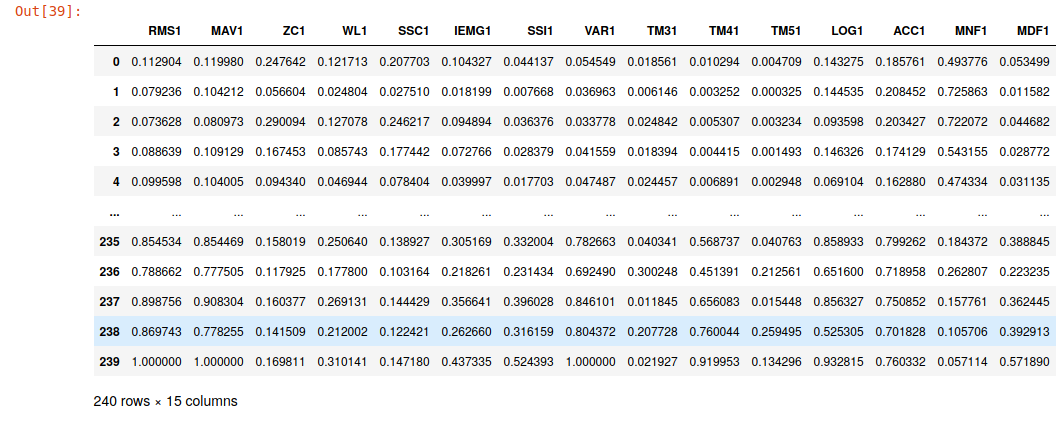
\includegraphics[scale=0.38]{imagenes/datos canal 1.png}
            \caption{Archivo entrenamiento-testeo del canal 1}
            \label{fig:archivo1}
        \end{figure}
        
        \subsubsection{Canal 2}
        
        \begin{figure}[ht]
            \centering
            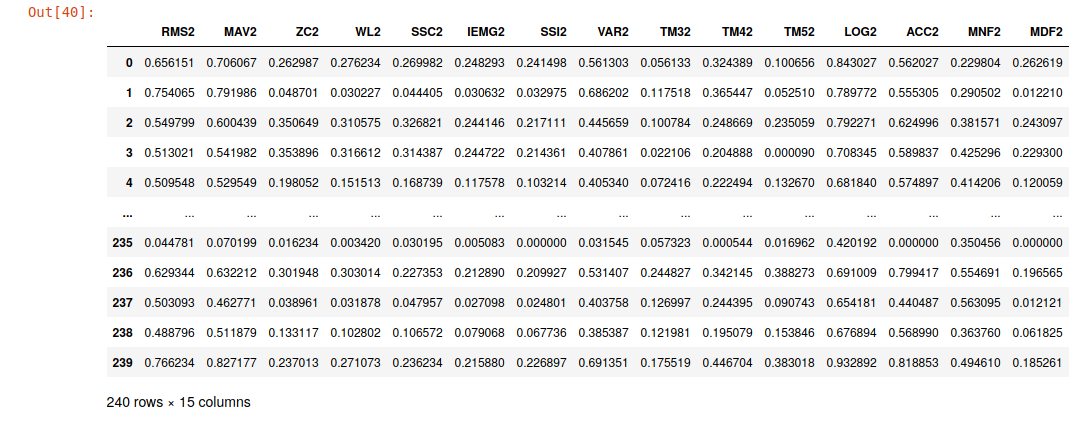
\includegraphics[scale=0.4]{imagenes/datos canal 2.png}
            \caption{Archivo entrenamiento-testeo del canal 2}
            \label{fig:archivo2}
        \end{figure}
        
        \subsubsection{Canal 3}
        \begin{figure}[ht]
            \centering
            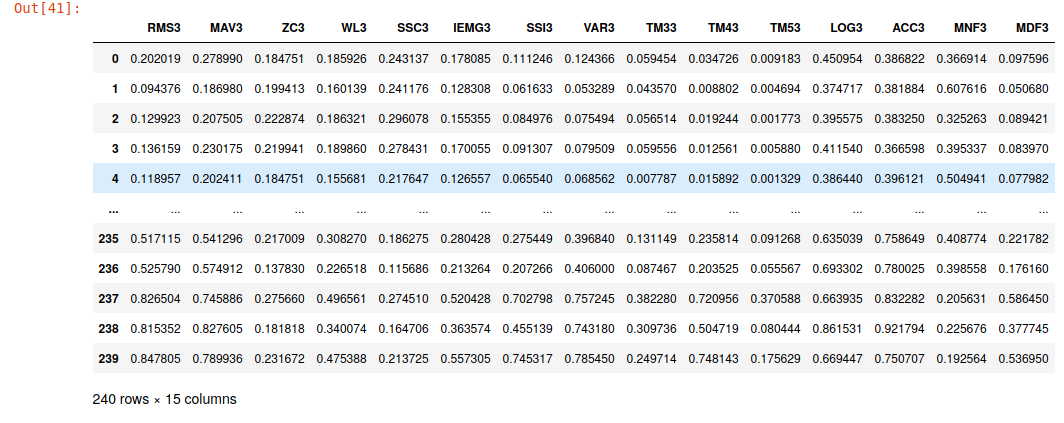
\includegraphics[scale=0.4]{imagenes/datos canal 3.png}
            \caption{Archivo entrenamiento-testeo del canal 3}
            \label{fig:archivo3}
        \end{figure}
        
        
        \subsubsection{Canal 4}
        \begin{figure}[ht]
            \centering
            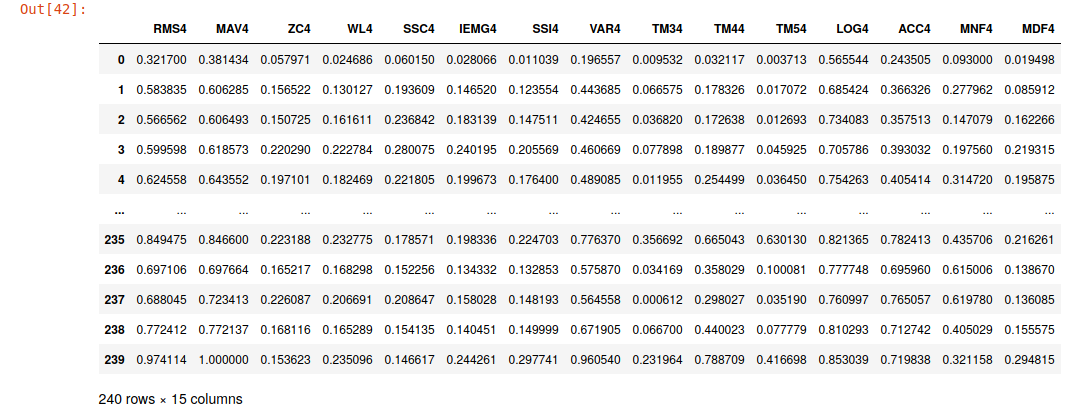
\includegraphics[scale=0.4]{imagenes/datos canal 4.png}
            \caption{Archivo entrenamiento-testeo del canal 4}
            \label{fig:archivo4}
        \end{figure}
        
        \newpage
        \subsubsection{Canal 1,2}
        \begin{figure}[ht]
            \centering
            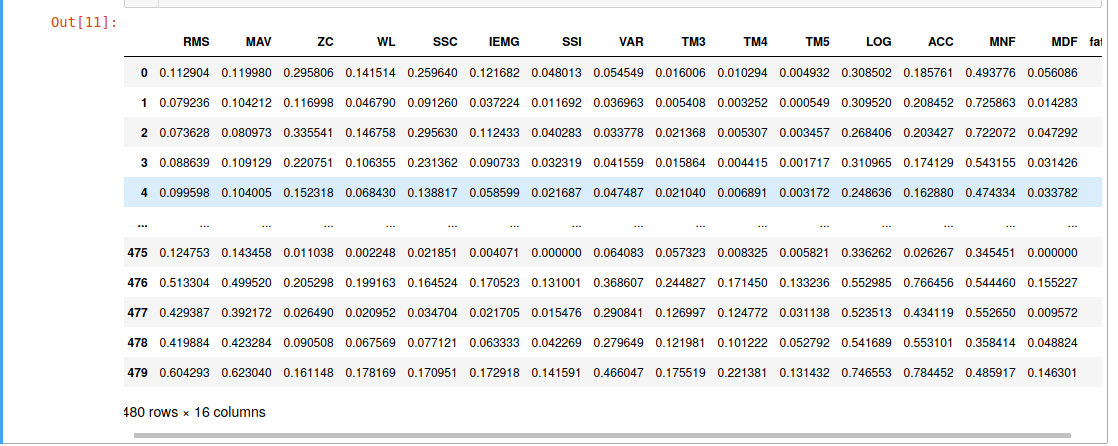
\includegraphics[scale=0.4]{imagenes/datos canal12.png}
            \caption{Archivo entrenamiento-testeo del canal 1,2}
            \label{fig:archivo12}
        \end{figure}
        
      
        \subsubsection{Canal 3,4}
        \begin{figure}[ht]
            \centering
            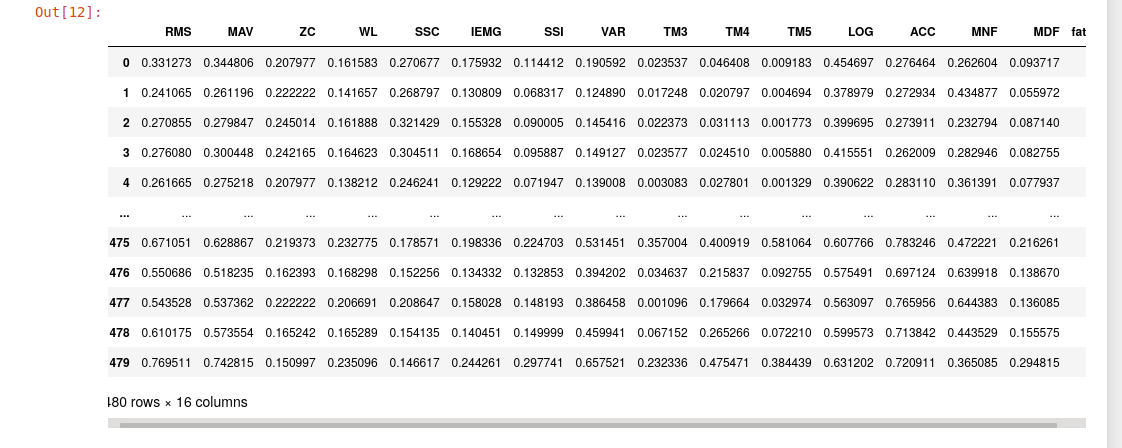
\includegraphics[scale=0.4]{imagenes/datos canal 34.png}
            \caption{Archivo entrenamiento-testeo del canal 3,4}
            \label{fig:archivo34}
        \end{figure}
        
        
        \newpage
        \subsubsection{Canal Total}
        \begin{figure}[ht]
            \centering
            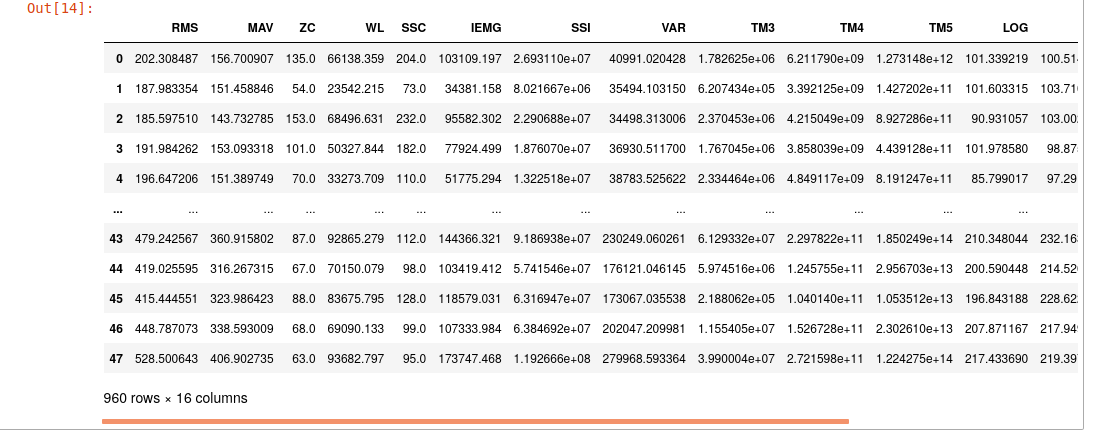
\includegraphics[scale=0.4]{imagenes/datos canal total.png}
            \caption{Archivo entrenamiento-testeo del canal total}
            \label{fig:archivototal}
        \end{figure}
    
    
    \subsection{Estimación de fatiga}
    La estimación de fatiga es calculada a la hora de crear los archivos de entrenamiento-testeo. Aquí se muestra como se iba calculando el array de etiquetas de cada uno de los archivos EMG utilizados.
    \begin{figure}[ht]
            \centering
            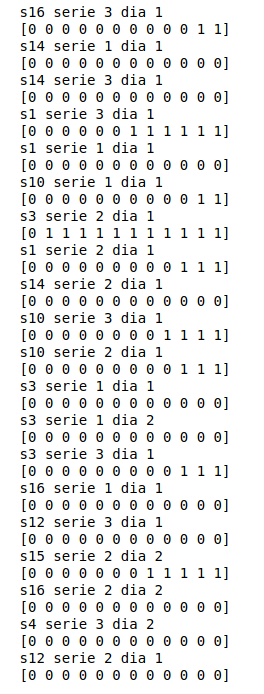
\includegraphics[scale=0.3]{imagenes/estimacion fatiga.png}
            \caption{Calculo de la fatiga}
            \label{fig:calculo fatiga}
    \end{figure}
    
    \subsection{Selección de características: RFE}
    Esta sección va dedicada a mostrar, las características elegidas para el archivo de entrenamiento-testeo de cada uno de los canales estudiados. Se mostrara en cada canal el numero de características finales (1,2 y 5).
        \subsubsection{Canal 1, Canal 2, Canal 3 y Canal 4 todos con N = 1} 
        \begin{figure}[ht]
            \centering
            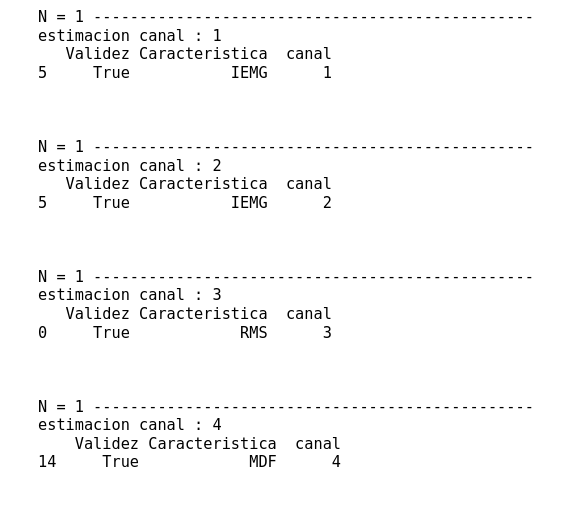
\includegraphics[scale=0.3]{imagenes/N1 canales 1234.png}
            \caption{RFE con N=1 aplicado al canal 1, canal 2, canal 3 y canal 4}
            \label{fig:N1 canal 1234}
        \end{figure}
        
        \subsubsection{Canal 1, Canal 2, Canal 3 y Canal 4 todos con N = 2} 
        \begin{figure}[ht]
            \centering
            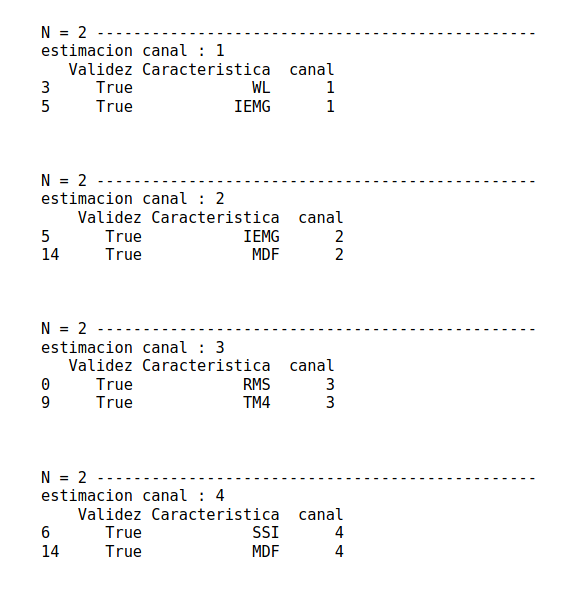
\includegraphics[scale=0.3]{imagenes/N2 canales 1234.png}
            \caption{RFE con N=2 aplicado al canal 1, canal 2, canal 3 y canal 4}
            \label{fig:N2 canal 1234}
        \end{figure}
        
        \subsubsection{Canal 1, Canal 2, Canal 3 y Canal 4 todos con N = 5} 
        \begin{figure}[ht]
            \centering
            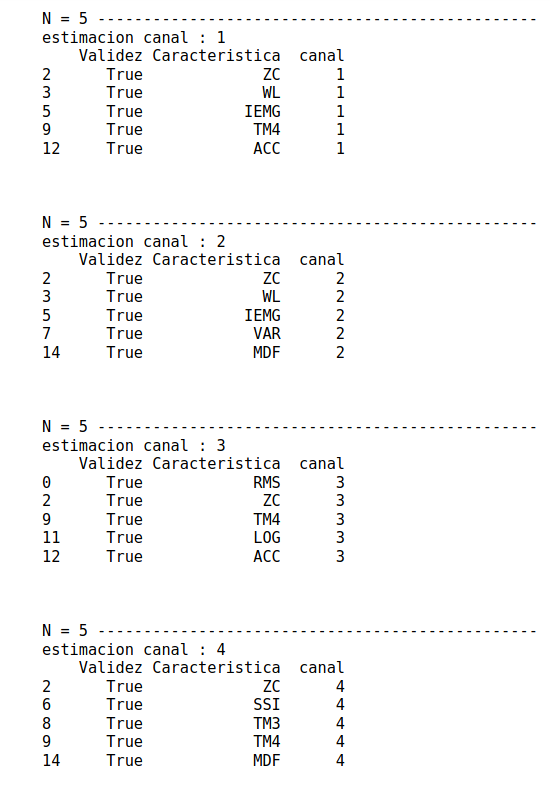
\includegraphics[scale=0.25]{imagenes/N5 canales 1234.png}
            \caption{RFE con N=5 aplicado al canal 1, canal 2, canal 3 y canal 4}
            \label{fig:N5 canal 1234}
        \end{figure}
        
        
        \newpage
        \subsubsection{Canal 1,2 con N = 1, 2 y 5}
        \begin{figure}[ht]
            \centering
            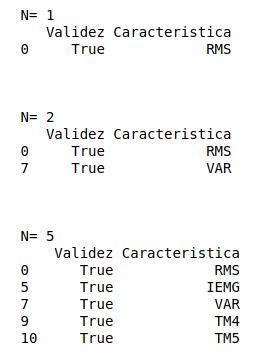
\includegraphics[scale=0.3]{imagenes/RFE canal 12.png}
            \caption{RFE con N=1, 2 y 5 aplicado al canal 1,2 }
            \label{fig:REF canal 12}
        \end{figure}
        
        \subsubsection{Canal 3,4 con N = 1, 2 y 5}
        \begin{figure}[ht]
            \centering
            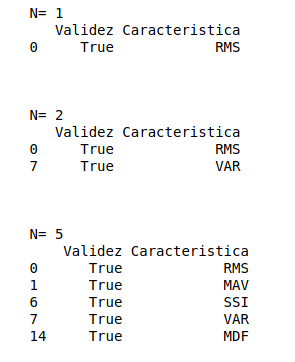
\includegraphics[scale=0.3]{imagenes/RFE canal 34.png}
            \caption{RFE con N=1, 2 y 5 aplicado al canal 3,4 }
            \label{fig:REF canal 34}
        \end{figure}
        
        
        \subsubsection{Canal Total con N = 1, 2 y 5}
        \begin{figure}[ht]
            \centering
            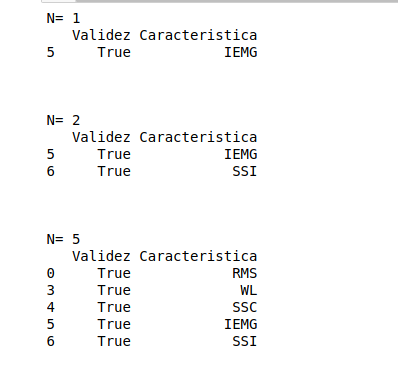
\includegraphics[scale=0.3]{imagenes/RFE canal total.png}
            \caption{RFE con N=1, 2 y 5 aplicado al canal total}
            \label{fig:REF canal total}
        \end{figure}
        
        
        
        
        
        
        
        
        
        
        
        \begin{table}[!ht]
    \centering
    \caption{Desviación típica de los clasificadores en cada canal}
    \vspace{0.5cm}
    \scalebox{0.63}{
            \begin{tabular}{lllll}
            \toprule
                      &     &        N = 1 &        N = 2 &        N = 5 \\
            \midrule
            \multirow{\textbf{canal 1}} & \textbf{SVM} &  0.0482327 &  0.0482327 &  0.0306186 \\
                      & \textbf{TREE} &  0.0980717 &   0.108653 &   0.132419 \\
                      & \textbf{KNN} &  0.0520416 &  0.0482327 &  0.0709558 \\
            \cline{1-5}
            \multirow{\textbf{canal 2}} & \textbf{SVM} &   0.083749 &   0.108173 &   0.107529 \\
                      & \textbf{TREE} &   0.111492 &   0.101208 &   0.119606 \\
                      & \textbf{KNN} &  0.0386401 &  0.0372678 &  0.0448764 \\
            \cline{1-5}
            \multirow{\textbf{canal 3}} & \textbf{SVM} &  0.0306186 &  0.0372678 &  0.0980717 \\
                      & \textbf{TREE} &  0.0991281 &  0.0853913 &  0.0953794 \\
                      & \textbf{KNN} &  0.0408248 &  0.0386401 &  0.0752311 \\
            \cline{1-5}
            \multirow{\textbf{canal 4}} & \textbf{SVM} &   0.125968 &   0.130437 &  0.0276385 \\
                      & \textbf{TREE} &  0.0903312 &  0.0953794 &   0.129502 \\
                      & \textbf{KNN} &  0.0372678 &  0.0311805 &  0.0603807 \\
            \cline{1-5}
            \multirow{\textbf{canal total}} & \textbf{SVM} &  0.0660124 &  0.0661602 &  0.0304409 \\
                      & \textbf{TREE} &  0.0593476 &  0.0721237 &   0.053966 \\
                      & \textbf{KNN} &  0.0169891 &  0.0295731 &  0.0364732 \\
            \cline{1-5}
            \multirow{\textbf{canal 1,2}} & \textbf{SVM} &     0.0125 &       0.05 &   0.128695 \\
                      & \textbf{TREE} &   0.052125 &  0.0557462 &   0.077784 \\
                      & \textbf{KNN} &  0.0186339 &  0.0186339 &  0.0315953 \\
            \cline{1-5}
            \multirow{\textbf{canal 3,4}} & \textbf{SVM} &     0.0125 &     0.0125 &     0.0125 \\
                      & \textbf{TREE} &  0.0682749 &   0.052125 &  0.0764331 \\
                      & \textbf{KNN} &    0.01932 &  0.0222439 &  0.0320048 \\
            \bottomrule
            \end{tabular}
    }
\end{table}